\documentclass[10pt,letterpaper]{article}
\usepackage[margin=.82in]{geometry}
\usepackage{amsmath,amssymb,amsthm,booktabs,graphicx}
\usepackage[hidelinks]{hyperref}
\newtheorem{theorem}{Theorem}
\newcommand{\K}{\operatorname{sf}}
\newcommand{\vp}{\nu}
\title{Almost primes in square products of factorials}
\author{Pioneer project}
\date{28 November 2026}
\begin{document}
\begin{center}
{\Large\bfseries Almost primes in square products of factorials}\par\smallskip
Pioneer project \quad 28 November 2026
\end{center}
\begin{abstract}
Erd\H{o}s and Graham conjectured that almost every product of two primes is absent from the endpoints of square products of at most five distinct factorials. We prove that for each fixed \(k\ge2\), almost every integer with \(k\) prime factors counted with multiplicity requires exactly six factorials. A uniform Brun--Titchmarsh estimate on shifted almost primes allows us to apply a structural theorem of Yudin. We also answer Chai Wah Wu's finite question about the first endpoint with at least four prime factors admitting no five-factorial representation: it is \(435643=13\cdot23\cdot31\cdot47\). Two reproducible computations verify minimality.
\end{abstract}

\section{The relative density of six-factorial endpoints}

For \(n\ge2\), let \(F(n)\) be the least \(j\ge2\) for which
\(1\le b_1<\cdots<b_j=n\) and \(\prod_i b_i!\) is a square; set \(F(n)=\infty\) when there is no such representation. Write \(D_j=\{n:F(n)=j\}\) and let \(\Omega(n)\) count prime factors with multiplicity. Erd\H{o}s and Graham showed that almost all endpoints \(13p\), with \(p\) prime, lie outside their set of endpoints representable with at most five factorials. They conjectured the same when both primes vary \cite[Theorem~3 and p.~353]{eg}. OEIS A389148 records the version excluding exactly five factorials \cite{parent}. Our result implies both formulations.

\begin{theorem}\label{thm:almost}
For each fixed integer \(k\ge2\),
\[
\lim_{x\to\infty}
 \frac{\#\{n\le x:\Omega(n)=k,\ F(n)=6\}}
      {\#\{n\le x:\Omega(n)=k\}}=1 .
\]
In particular almost every semiprime belongs to A389148.
\end{theorem}

Let \(s(v)=\prod_{\nu_q(v)\text{ odd}}q\) be the squarefree part of \(v\), and let \(P(v)\) denote the largest prime divisor of \(v\), with \(P(1)=1\). Yudin's Corollary~6.2 \cite{yudin} states that, for each fixed \(0<\varepsilon\le10^{-3}\), all but at most \(X^{1/2+6\varepsilon+o(1)}\) squarefree \(n\in(X/2,X]\) satisfying
\[
 P(n)>X^{1-\varepsilon/2},\qquad P(s(n-1))>X^{3\varepsilon}
 \tag{1}\label{eq:hyp}
\]
have no representation with fewer than five factorials. Every five-factor representation of such an \(n\) consists of \(n!, (n-1)!,m!,(m-1)!,c!\) with \(n-1>m>m-1>c\ge1\). Its exceptional bound is smaller than the counting function of every fixed \(k\)-almost-prime family. Obtaining the second condition in \eqref{eq:hyp} on that family requires a relative estimate.

\paragraph{Removing atypical factorizations.}
Write \(I_X=(X/2,X]\) and \(H_k(X)=X(\log\log X)^{k-1}/\log X\).
Landau's theorem for \(k\)-almost primes, with and without repeated factors \cite{wright}, gives
\[
 \#\{n\in I_X:\Omega(n)=k\}\sim \frac{H_k(X)}{2(k-1)!}.
\]
The same asymptotic holds for squarefree \(n\), so repeated factors cost \(o_k(H_k(X))\). We henceforth write \(n=ap\), where \(p=P(n)\) is prime and \(a\) is the product of the \(k-1\) other primes. Fix an integer \(B\), to be chosen in terms of \(k\). We may impose
\[
  r>B\quad\text{for all }r\mid a\text{ prime},\qquad a\le X^{\varepsilon/4}
  \tag{2}\label{eq:cofactor}
\]
at a cost of \(O_{k,B,\varepsilon}(H_k(X)/\log\log X)\).
Indeed, for each possible \(a\) we have \(X/a\ge p>(X/2)^{1/k}\), so the number of choices of \(p\) is \(O_k(X/(a\log X))\). If \(a>X^{\varepsilon/4}\), at least one of its prime factors exceeds \(X^\delta\), with \(\delta=\varepsilon/(4(k-1))\).
Mertens' estimate \(\sum_{r\le t}1/r=\log\log t+O(1)\), over primes, gives an \(O_\delta(1)\) reciprocal sum on \((X^\delta,X]\); the reciprocal sum over \(r\le B\) is also bounded. Each of the other \(k-2\) prime factors costs \(O(\log\log X)\), proving the asserted error. Under \eqref{eq:cofactor} one has \(p>X/(2a)\ge X^{1-\varepsilon/4}/2>X^{1-\varepsilon/2}\) for sufficiently large \(X\).

\paragraph{Large prime factors of the shifted squarefree part.}
Set \(y=X^{3\varepsilon}\) and
\[
 W(n)=\sum_{\substack{\ell\le y,\ \ell\mid n-1\\ \ell\ {\rm prime}}}\log\ell.
\]
Write \(n-1=u^2s(n-1)\). There are \(O(X^{3/4})\) endpoints with \(u>X^{1/4}\): sum \(X/u^2\) over \(X^{1/4}<u\le\sqrt X\). Otherwise \(s(n-1)\ge\sqrt X/3\) for large \(X\). If \(P(s(n-1))\le y\), all primes in that squarefree number occur in \(W(n)\), whence \(W(n)\ge\log(\sqrt X/3)\).

For a fixed \(a\) from \eqref{eq:cofactor} and a prime \(\ell\le y\), the condition \(\ell\mid ap-1\) is impossible if \(\ell\mid a\). Otherwise \(p\equiv a^{-1}\pmod\ell\). Put \(T=X/a\). The Brun--Titchmarsh inequality \cite[Theorem~2]{mv} gives
\[
 \#\{p\le T:p\equiv a^{-1}\pmod\ell\}
 \le \frac{2T}{(\ell-1)\log(T/\ell)}
 \ll \frac{X}{a(\ell-1)\log X}.
\]
Here \(T/\ell\ge X^{1-13\varepsilon/4}\), so the implied constant is absolute over the entire interval \(0<\varepsilon\le10^{-3}\). Summing first over \(\ell\), then over \(a\), bounds the sum of \(W(n)\) over the retained endpoints by
\[
 \frac{O(X)}{\log X}
 \left(\sum_{a}\frac1a\right)
 \left(\sum_{\ell\le y}\frac{\log\ell}{\ell-1}\right)
 \ll_k \varepsilon X(\log\log X)^{k-1}.
\]
Indeed, the first sum is at most the \((k-1)\)-st power of the reciprocal-prime sum, and the second prime sum is \(O(\log y)\) by partial summation from Chebyshev's bound. Dividing by \(\log(\sqrt X/3)\) shows that at most \(C_k\varepsilon H_k(X)+O(X^{3/4})\) retained endpoints fail the second condition of \eqref{eq:hyp}. The constant \(C_k\) is independent of \(\varepsilon\).

\paragraph{Excluding the two consecutive pairs.}
For \(s_c=s(c!)\), every prime in \((c/2,c]\) occurs once in \(c!\). The prime number theorem therefore gives \(\log s_c\ge(1/2+o(1))c\). Choose \(B=B(k)\) so that \(s_c>c^{2(k-1)}\) for all \(c\ge B\). For squarefree \(a\) from \eqref{eq:cofactor},
\[
 s(a\,c!)=\frac{a s_c}{\gcd(a,s_c)^2}\ \ge a\qquad(c\ge0).
 \tag{3}\label{eq:rigid}
\]
When \(c<B\), the gcd is one. For \(c\ge B\), every prime in the gcd is at most \(c\), and there are at most \(k-1\) of them.

Take a retained \(n=ap\) satisfying \eqref{eq:hyp} outside Yudin's exceptional set. A five-factor representation would require \(nm c!\) to be a square for some \(m<n\). Then \(s_c=s(nm)\le X^2\), so \(c=O(\log X)<p\). Since \(p\) occurs exactly once in \(n\), we have \(p\mid m\). Writing \(m=tp\) gives \(1\le t<a\) and \(a t c!\) square. This forces \(t=s(a c!)v^2\) for some integer \(v\ge1\), contradicting \eqref{eq:rigid}. Thus \(F(n)\ge6\) in the extended sense. The three adjacent pairs ending at \(a,p,n\) give six distinct factorials with square product, since \(apn=n^2\). They are distinct for large \(X\), as \(2\le a\le X^{\varepsilon/4}\) and \(p>X^{1-\varepsilon/2}\). Consequently \(F(n)=6\).

For each fixed \(\varepsilon\), the total number of exceptions in \(I_X\) is at most \(C_k\varepsilon H_k(X)+o_{k,\varepsilon}(H_k(X))\); the power saving in Yudin's theorem is sufficient for this estimate. Taking a limsup and then letting \(\varepsilon\) decrease to zero gives relative density one on dyadic intervals. For any given error proportion, sum this bound over the dyadic intervals below \(x\) whose top endpoints exceed the corresponding threshold; the remaining initial interval is bounded. This proves Theorem~\ref{thm:almost}.

\section{The first endpoint with four or more prime factors}

Theorem~\ref{thm:almost} gives relative density one in each fixed factor-count family, without locating its first member. OEIS A392333 lists non-semiprime composite \(e\) for which exactly five distinct factorials with largest argument \(e\) cannot have square product. The first 657 tabulated terms are products of three distinct primes. Chai Wah Wu asked for the first term with \(\Omega(e)\ge4\) \cite{oeis}.

\begin{theorem}
Put \(E=435643\). Every \(e<E\) with \(\Omega(e)\ge4\) admits a square product of five distinct positive-index factorials ending in \(e!\). No such product exists at \(E\), and \(F(E)=6\). Consequently \(E\) is both the requested term of A392333 and the least member of \(D_6\) with \(\Omega(e)\ge4\).
\end{theorem}

\subsection{Earlier endpoints}

Continue to write \(\K(x)=s(x)\) for the squarefree kernel. For \(e=pm\) with least prime factor \(p\le11\), take five indices
\[
 t,\quad qm-1,\quad qm,\quad e-1,\quad e,
\]
with \((p,q,t)\) in the table. The square class of their factorial product is that of \(t!\,qm\,e=t!pq\,m^2\), which is a square in each row.
\[
\begin{array}{c|rrrrr}
p & 2&3&5&7&11\\
q & 1&2&1&5&7\\
t & 2&3&6&7&11\\
\K(t!) &2&6&5&35&77
\end{array}
\]
Since \(\Omega(e)\ge4\), \(m\ge p^3\), so \(t<qm-1\) and \(qm<e-1\) throughout. If \(p>11\) and \(e=r^2m\) for some prime \(r\), use \(1,m-1,m,e-1,e\). Here \(m\ge13^2\), and \(me=(rm)^2\). These two constructions cover 193,806 earlier endpoints. The remaining candidates are squarefree with at least four prime factors, all at least 13. There are 109 such candidates below \(E\). Each row of the companion witness table gives \(a,b,c,d\) for which \(a!b!c!d!e!\) is square.

The first candidate is \(96577=13\cdot17\cdot19\cdot23\). A witness uses the indices 5, 7, 23, 96576 and 96577. The verifier tests all prime exponents. Here the shorter check is \(\K(5!\,7!\,23!)=96577\).

\begin{figure}[ht]
\centering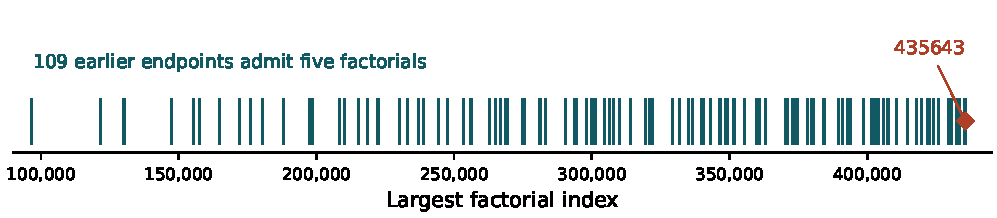
\includegraphics[width=.85\linewidth]{endpoints.pdf}
\caption{Every squarefree candidate with at least four prime divisors, all at least 13, through \(E\). The witness table certifies each vertical mark. The diamond is the first excluded endpoint.}
\end{figure}

\subsection{Exhaustive exclusion at the endpoint}

Two positive integers have the same square class exactly when their vectors of prime valuations modulo two agree. Fix \(e=E\) and suppose \(a<b<c<d<e\) gives a square. With \(P=435641\), the largest prime below \(e\), each factorial of index between \(P\) and \(e\) contains \(P\) once. Hence \(d\ge P\), leaving two cases. For each set \(Q=\K(e!/d!)\), put \(q\) equal to its largest prime factor. We must have \(c\ge q\), since \(a!b!c!\) has the square class of \(Q\).

For any \(c\ge3\) let \(r\) be the largest prime at most \(c\). Bertrand's postulate gives \(r>c/2\), so \(r\) has exponent one in \(c!\). If \(r>q\), then \(b\ge r\), since otherwise \(a!b!c!\) would have odd \(r\)-valuation. Thus it suffices to try
\[
 \max(3,q)\le c<d,\qquad
 b_0\le b<c,\qquad
 b_0=\begin{cases}r,&r>q,\\2,&r\le q.\end{cases}
\]
For each triple \((b,c,d)\), index the factorials \(a!\) by the parities of the first 64 prime valuations. Look up all \(1\le a<b\) that match the signature required for a square. For every match, test all primes \(p\le E\) using Legendre's formula \(\vp_p(n!)=\sum_{j\ge1}\lfloor n/p^j\rfloor\). Projection cannot discard a square. The exact counts are
\[
\begin{array}{r|l|r|r|r}
 d & \text{primes in }Q & (b,c)\text{ pairs} & a\text{ matches} & \text{squares}\\ \midrule
 435642 &13,23,31,47 &4\,029\,063&94&0\\
 435641 &2,3,13,17,23,31,47,4271 &4\,016\,263&90&0 .
\end{array}
\]
A second implementation forms the factorial signatures by sieving and maps each prime deterministically to a 64-bit vector. It applies the same necessary bounds and checks every surviving candidate against all prime valuations. Both enumerations independently produce a witness for each of the 109 earlier candidates and exclude \(E\).

\subsection{The minimum length at \(E\)}

The squarefree kernels in the table rule out a two-factorial square. A three-factorial square would require \(\K(a!)=Q\). Its largest prime \(q\) restricts \(a\) to the interval from \(q\) through the integer preceding the next prime, by Bertrand's postulate again. In the first row \(a=47,48,49,50,51,52\) fail at the primes \(3,23,23,2,2,2\), respectively. In the second row \(a=4271,4272\) both fail at \(2\). A four-factorial square containing \(1!\) would give a three-factorial square by removing it. Any other four-factorial square would give a five-factorial square by adjoining \(1!\).

The adjacent-pair construction of Erd\H{o}s and Graham \cite{eg}, also given in \cite[Eq.~(1.3)]{yudin}, supplies the six indices
\[
 12,\ 13,\ 33510,\ 33511,\ 435642,\ 435643.
\]
These form three adjacent pairs. Their product of factorials has the square class of
\(13\cdot33511\cdot435643=435643^2\). This proves \(F(E)=6\). Yudin determined the orders of growth asked for in Erd\H{o}s Problem 374 \cite{bloom,yudin}. The existence of a limiting natural density for \(D_6\) is a further open question \cite[Sec.~8]{yudin}.

\begin{thebibliography}{9}
\bibitem{oeis} C. W. Wu, OEIS A392333, 2026. \url{https://oeis.org/A392333}.
\bibitem{eg} P. Erd\H{o}s and R. L. Graham, \emph{On products of factorials}, Bulletin of the Institute of Mathematics, Academia Sinica 4 (1976), 337--355. \url{https://users.renyi.hu/~p_erdos/1976-25.pdf}.
\bibitem{bloom} T. F. Bloom, \emph{Erd\H{o}s Problem 374}. \url{https://www.erdosproblems.com/374}.
\bibitem{parent} C. W. Wu, OEIS A389148, 2025. \url{https://oeis.org/A389148}.
\bibitem{wright} E. M. Wright, \emph{A simple proof of a theorem of Landau}, Proceedings of the Edinburgh Mathematical Society 9 (1954), 87--90. \url{https://doi.org/10.1017/S0013091500021349}.
\bibitem{mv} H. L. Montgomery and R. C. Vaughan, \emph{The large sieve}, Mathematika 20 (1973), 119--134. \url{https://doi.org/10.1112/S0025579300004708}.
\bibitem{yudin} F. Yudin, \emph{Square products of factorials and a conjecture of Erd\H{o}s and Graham}, arXiv:2610.01899, 2026. \url{https://arxiv.org/abs/2610.01899}.
\end{thebibliography}
\end{document}
